\documentclass{standalone}
\usepackage{tikz}
\usepackage{ctex,siunitx,ninecolors}
\setCJKmainfont{Noto Serif CJK SC}
\usepackage{tkz-euclide}
\usepackage{amsmath,mhchem}
\usetikzlibrary{patterns, calc}
\usetikzlibrary {decorations.pathmorphing, decorations.pathreplacing, decorations.shapes}
\begin{document}
\small
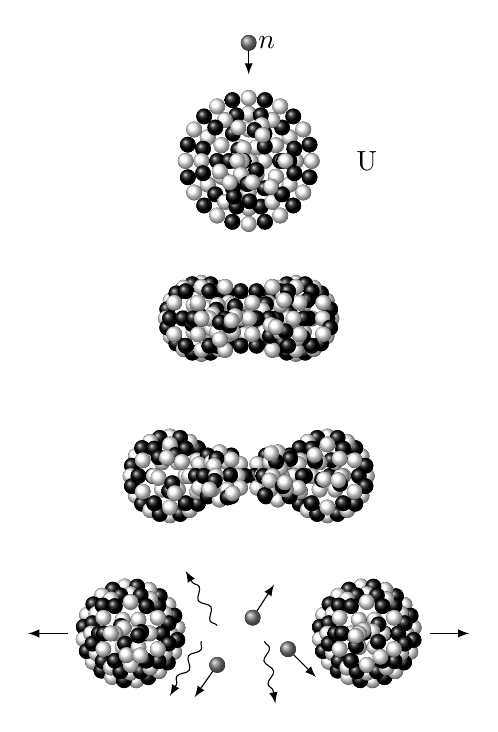
\begin{tikzpicture}[>=latex,scale=1.0]
  % \useasboundingbox(-1,1.2)rectangle(5,2.8);
  \draw[->](0,1.5)--(0,1.1);
  \fill[ball color=gray](0,1.5)circle(0.1)node[right]{$n$};
  \foreach \x in {0,60,...,300}
  {
    \fill[ball color=white](\x:0.8)circle(0.1);
    \fill[ball color=white](\x+30:0.8)circle(0.1);
    \fill[ball color=black](\x+15:0.8)circle(0.1);
    \fill[ball color=black](\x+45:0.8)circle(0.1);
    \fill[ball color=white](\x:0.6)circle(0.1);
    \fill[ball color=white](\x+30:0.6)circle(0.1);
    \fill[ball color=black](\x+45:0.6)circle(0.1);
    \fill[ball color=black](\x+15:0.6)circle(0.1);
    \fill[ball color=black](\x:0.4)circle(0.1);
    \fill[ball color=white](\x+30:0.4)circle(0.1);
    \fill[ball color=white](\x:0.2)circle(0.1);
    \fill[ball color=black](\x:0.75*rnd)circle(0.1);
    \fill[ball color=white](\x:0.75*rnd)circle(0.1);
    \fill[ball color=black](\x:0.55*rnd)circle(0.1);
    \fill[ball color=white](\x:0.55*rnd)circle(0.1);
  }
  \node at (1.5,0) {\ce{U}};
  \foreach \x in {0.6,-0.6}
  {
    \begin{scope}[xshift=\x cm,yshift=-2cm]
    \foreach \w in {0,60,...,300}
      {
        \fill[ball color=white](\w:0.45)circle(0.1);
        \fill[ball color=white](\w+30:0.45)circle(0.1);
        \fill[ball color=black](\w+45:0.45)circle(0.1);
        \fill[ball color=black](\w+15:0.45)circle(0.1);
        \fill[ball color=black](\w:0.4)circle(0.1);
        \fill[ball color=white](\w+30:0.4)circle(0.1);
        \fill[ball color=white](\w:0.2)circle(0.1);
        \fill[ball color=black](\w:0.35*rnd)circle(0.1);
        \fill[ball color=white](\w:0.35*rnd)circle(0.1);
      }
    \end{scope}
  }
  \foreach \x in {0.3,-0.3}
  {
    \begin{scope}[xshift=\x cm,yshift=-2cm]
    \foreach \w in {0,60,...,300}
      {
        % \fill[ball color=white](\w:0.45)circle(0.1);
        % \fill[ball color=white](\w+30:0.45)circle(0.1);
        % \fill[ball color=black](\w+45:0.45)circle(0.1);
        % \fill[ball color=black](\w+15:0.45)circle(0.1);
        \fill[ball color=black](\w:0.4)circle(0.1);
        \fill[ball color=white](\w+30:0.4)circle(0.1);
        \fill[ball color=white](\w:0.2)circle(0.1);
        \fill[ball color=black](\w:0.35*rnd)circle(0.1);
        \fill[ball color=white](\w:0.35*rnd)circle(0.1);
      }
    \end{scope}
  }
  \foreach \x in {1.0,-1.0}
  {
    \begin{scope}[xshift=\x cm,yshift=-4cm]
    \foreach \w in {0,60,...,300}
      {
        \fill[ball color=white](\w:0.5)circle(0.1);
        \fill[ball color=white](\w+30:0.5)circle(0.1);
        \fill[ball color=black](\w+45:0.5)circle(0.1);
        \fill[ball color=black](\w+15:0.5)circle(0.1);
        \fill[ball color=black](\w:0.4)circle(0.1);
        \fill[ball color=white](\w+30:0.4)circle(0.1);
        \fill[ball color=white](\w:0.2)circle(0.1);
        \fill[ball color=black](\w:0.35*rnd)circle(0.1);
        \fill[ball color=white](\w:0.35*rnd)circle(0.1);
      }
    \end{scope}
  }
  \foreach \x in {0.37,-0.37}
  {
    \begin{scope}[xshift=\x cm,yshift=-4cm]
    \foreach \w in {0,60,...,300}
      {
        \fill[ball color=black](\w:0.3)circle(0.1);
        \fill[ball color=white](\w+30:0.3)circle(0.1);
        \fill[ball color=white](\w:0.2)circle(0.1);
        \fill[ball color=black](\w:0.35*rnd)circle(0.1);
        \fill[ball color=white](\w:0.35*rnd)circle(0.1);
      }
    \end{scope}
  }
  \foreach \x in {1.5,-1.5}
  {
    \begin{scope}[xshift=\x cm,yshift=-6cm]
      \foreach \y in {0,60,...,300}
    {
      \fill[ball color=white](\y+7:0.6)circle(0.1);
      \fill[ball color=white](\y+37:0.6)circle(0.1);
      \fill[ball color=black](\y+52:0.6)circle(0.1);
      \fill[ball color=black](\y+22:0.6)circle(0.1);
      \fill[ball color=white](\y:0.5)circle(0.1);
      \fill[ball color=white](\y+30:0.5)circle(0.1);
      \fill[ball color=black](\y+45:0.5)circle(0.1);
      \fill[ball color=black](\y+15:0.5)circle(0.1);
      \fill[ball color=black](\y:0.4)circle(0.1);
      \fill[ball color=white](\y+30:0.4)circle(0.1);
      \fill[ball color=white](\y:0.2)circle(0.1);
      \fill[ball color=black](\y:0.35*rnd)circle(0.1);
      \fill[ball color=white](\y:0.35*rnd)circle(0.1);
    }
    \end{scope}
  }
  \draw[->](-2.3,-6)--(-2.8,-6);
  \draw[->](2.3,-6)--(2.8,-6);
  \draw[->](0.5,-6.2)--++(-45:0.5);
  \draw[->](-0.4,-6.4)--++(-125:0.5);
  \draw[->](0.05,-5.8)--++(57:0.5);
  \draw[->,decorate,decoration={snake,segment length=3mm,amplitude=.5mm,post length=1mm}](-0.4,-5.9)--++(120:0.8);
  \draw[->,decorate,decoration={snake,segment length=3mm,amplitude=.5mm,post length=1mm}](-0.6,-6.1)--++(-120:0.8);
  \draw[->,decorate,decoration={snake,segment length=3mm,amplitude=.5mm,post length=1mm}](0.2,-6.1)--++(-80:0.8);
  \foreach \x/\y in {0.5/-6.2,-0.4/-6.4,0.05/-5.8}
  {
    \fill[ball color=gray](\x,\y)circle(0.1);
  }
\end{tikzpicture}
\end{document}